\documentclass[11pt]{report}

\usepackage[T2A]{fontenc}
\usepackage[utf8x]{inputenc}
\usepackage[english, russian]{babel}

\usepackage[T1]{fontenc}
\usepackage{titlesec, blindtext, color}
\usepackage[left=3cm, right=3cm, bottom=4cm, top=3cm, bindingoffset=0cm]{geometry}

\usepackage{amsmath}
\usepackage{mathtext}
\usepackage{environ}

\usepackage{wrapfig}
\usepackage{graphicx}
\usepackage{caption}
\usepackage{subcaption}
\usepackage{tabularx}


\graphicspath{{img/}}

\definecolor{gray75}{gray}{0.75}
\newcommand{\hsp}{\hspace{20pt}}
\addto\captionsrussian{\renewcommand{\contentsname}{Содержание}}

\titleformat{\chapter}[hang]{\Huge\bfseries}{\thechapter\hsp\textcolor{gray75}{|}\hsp}{0pt}{\Huge\bfseries}


\newenvironment{itemize*}%
  {\begin{itemize}%
    \setlength{\itemsep}{2pt}%
    \setlength{\parskip}{0.75pt}}%
  {\end{itemize}}


\newenvironment{enumerate*}%
  {\begin{enumerate}%
    \setlength{\itemsep}{2pt}%
    \setlength{\parskip}{0.75pt}}%
  {\end{enumerate}}

\newcolumntype{R}{>{\rule{0pt}{0.55cm}\raggedleft\arraybackslash}X}%
\newcolumntype{L}{>{\rule{0pt}{0.55cm}\raggedright\arraybackslash}X}%
\newcolumntype{C}{>{\rule{0pt}{0.55cm}\centering\arraybackslash}X}%
\newcolumntype{P}{>{\rule{0pt}{0.55cm}\centering\hsize=\dimexpr2\hsize+2\tabcolsep+\arrayrulewidth\relax}X}%

\newenvironment{wrapfigure*}%
 {%
  \setlength{\columnsep}{15pt}%
  \wrapfloat{figure}}%
 {\endwrapfloat}


\NewEnviron{myequation}{%
\begin{equation}
\scalebox{1.5}{$\BODY$}
\end{equation}
}



\title{
	\textbf{Escapy2.0 Engine\\Short Specification and User Guide}
}
\author{Генрих Тимур Домагальски}
\date{31.07.2017 Издаине 1}



\begin{document}

\maketitle

\tableofcontents

\newpage

\chapter*{О движке}
Escapy2 это игровой движок написанный на java с использованием библиотек Dagger1, libGDX и Gson. Поскольку libGDX является лишь низкоуровневой оберткой над lwjgl - движок дает полноту простора в использовании openGL, в свою очередь Dagger делает код более модульным и масштабируемым. На момент издания этого документа, движок состоит из пяти ключевых пакетов: \begin{enumerate*}
	\item Context
	\item Desktop
	\item Graphic
	\item Group
	\item Utils
\end{enumerate*}
Каждому из вышеперечисленных пакетов посвящена отдельная глава, подробнее со структурой api можно ознакомится через javadoc. На конец следует сразу заметить, что данный документ, так же как и сам движок расчитан на разработчиков неплохо знакомых с java и ООП, а так же основами openGL. Основной задачей документа не является скурпулезное описание API - за этим следует идти в javadoc, основная же цель документа - в первую очередь кратко обрисовать возможности движка, его принцип работы, а так же life-cycle и тп.


\chapter{Начало работы}
Вход производится похожим образом как в libGDX и lwjgl - в main с созданием инстанции
\textbf{LwjglApplication}. Для этого создается объект \textbf{LwjglApplicationConfiguration} который загружается из json файла с помощью 
\textbf{EscapyDesktopConfigLoader}, о самих загрузчиках и механизме сериализации в движке более подробно потом. 
\begin{center}
	
\includegraphics[width=1.25\linewidth]{img/1.png} 
  	\label{img:12}
  	  	
  	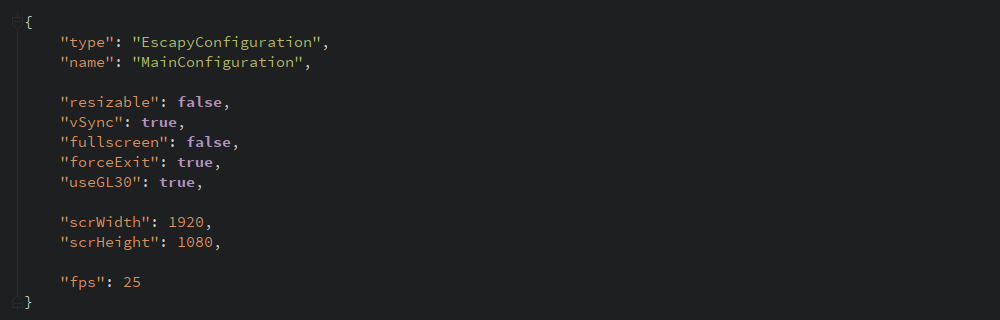
\includegraphics[width=1.25\linewidth]{img/2.png}   	
\end{center}
При создании \textbf{LwjglApplication} в качестве аргумента передается\\
\textbf{EscapyApplicationAdapter}, который в свою очередь в качестве аргумента принимает класс наследующийся от \textbf{EscapyGameContext} и varargs модулей Dagger'a.
\begin{center}
	
\includegraphics[width=1.25\linewidth]{img/3.png} 
  	\label{img:3} 
\end{center}
Подробнее о том как использовать модули Dagger'a можно прочитать на оффициальном  сайте проекта (\textit{http://square.github.io/dagger/}). \textbf{EscapyGameContext} имеет два конструктора, один из них как аргумент принимает инстанцию класса унаследованного от
\textbf{EscapyGameContextConfiguration} - абстрактного класса предоставляющего конфигурацию проекта через методы которые можно перегрузить в случае необходимости.
\begin{center}
	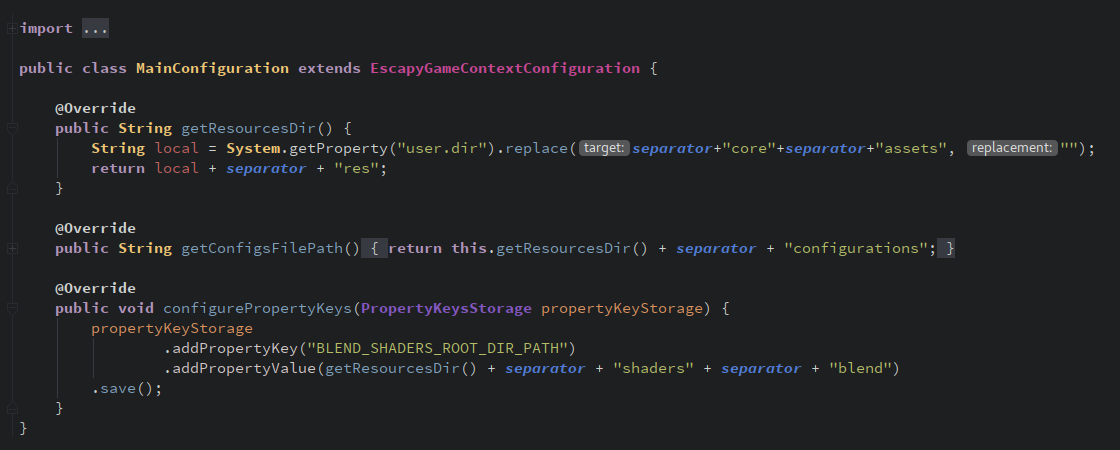
\includegraphics[width=1.2\linewidth]{img/4.png} 
  	\label{img:4} 
\end{center}


\chapter{Context}
Самый главный и значимый пакет движка в плане его архитектуры. Его основными элементами
являются два субпакета - \textit{\textbf{game}} и \textit{\textbf{annotation}} и класс
\textit{\textbf{EscapyGameContext}}. Последний наследуется от интерфейса \textit{\textbf{EscapyScreenContext}} позволяя тем самым на работу с экранами (сценами).

\section{Game}
Основные эллементы данного субпакета это классы: \begin{itemize*}
\item EscapyGameContextConfiguration - абстрактный класс делегирующий настройки
\item EscapyScreenContext - интерфейс управления экранами
\item EscapyScreen - интерфейс экрана (сцены).
\item PropertyKeysStorage - интерфейс позволяет сохранять пары ключ-объект.
\item Escapy - синглетон хранящий некоторые настройки.
\\
\end{itemize*}
\subsection*{EscapyScreen}
Отдельного внимания заслуживает этот интерфейс, он в свою очередь наследуется от интерфейса \textit{\textbf{Screen}} из библиотеки libGDX и содержит callback методы в которых должна находиться логика игры. Класс реализующий данный интерфейс, может (опционально) быть отмечен аннотацией \textit{\textbf{@SreenName("...")}}, в таком случае этому экрану будет присвоенно имя с помощью которого к этому экрану можно будет обращаться через методы интерфейса \textit{\textbf{EscapyScreenContext}}.

\section{Annotation}
Cодержит аннотации такие как \textit{\textbf{@SreenName("...")}}, а так же субпакет 
\textit{\textbf{meta}} содержащий процессор аннотаций построенный по шаблону <<Декоратор>>. Если интересуют подробности или возникло желание написать свою собственную имплементацию, то лучшем решением будет отсылка в javadoc или исходники.



\chapter{Utils}
Пакет со вспомогательными классами и прочими полезными вещами. Особого внимания заслуживают: \begin{itemize*}
	
	\item \textit{\textbf{EscapyArray и EscapyAssociatedArray}} - интерфейсы (и их 				реализации) наследующие Iterable c массивом внутри.
	
	\item Пакет \textit{\textbf{proxy}} - позволяет инстацировать объекты с listener'ами 		внутри.
	
	\item \textit{\textbf{EscapyInstanceLoader}}  - позволяет инстанцировать объекты по 		имени с помощью аннотации \textit{\textbf{@EscapyInstanced("...")}} или по имени 			метода.

	\item \textit{\textbf{EscapySerialized и EscapySimpleSerialized}} - интерфейс и 			абстрактный класс реализующий этот интерфейс, служат шаблоном для сериализуемы с помщью
	Gson'a классов.
\end{itemize*}
	\newpage
\section{EscapySimpleSerialized}
Так выглядит этот шаблон в исходниках.
\begin{center}
	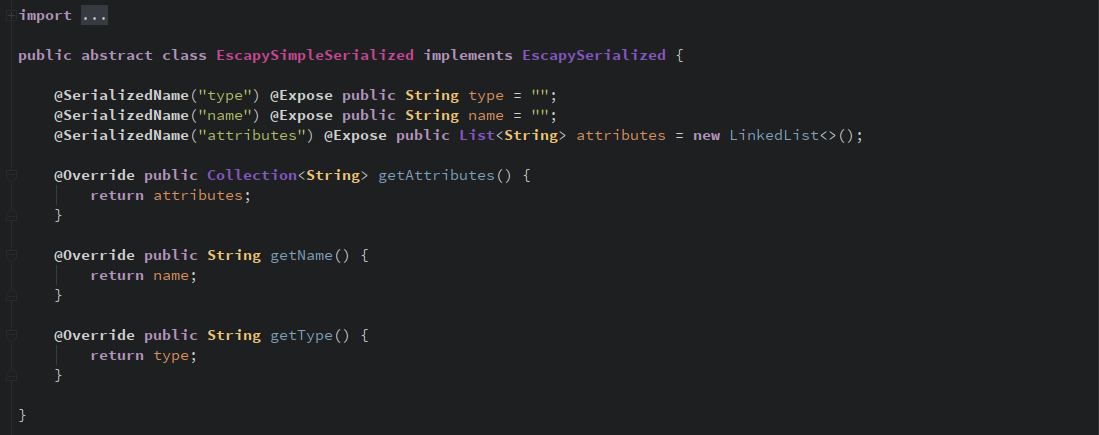
\includegraphics[width=1.2\linewidth]{img/5.png} 
  	\label{img:5} 
\end{center}	
А так выглядит его json.	
\begin{center}
	
\includegraphics[width=1.2\linewidth]{img/6.png} 
  	\label{img:6} 
\end{center}
Поскольку все классы движка должны сериализовываться через этот шаблон, код выше является необходимым минумом, для того что бы загрузчики движка могли успешно выполнить свою работу.
\newpage
\section{EscapyInstanceLoader}
Класс реализующий этот интерфейс позволяет на вызов инстанцирующих методов по имени либо самого метода, либо указанного в аннотации которым этот метод отмечен. Этот механизм очень удобен в использовании в загрузчиках движка и потому повсеместно там используется - для инстанцирования объектов по имени указаноому в json файле, либо для загрузки атрибутов для уже существующего объекта. 


\subsection{Загрузка аттрибутов}
Данный пример показывает как производить загрузку аттрибутов для уже существуюшего объекта - сначала создается класс реализующий интерфейс, затем инстанция класса передается в загрузчкик.
\begin{center}
	
\includegraphics[width=1.2\linewidth]{img/7.png} 
  	\label{img:7} 
\end{center}
И в загрузчкие, во время инициализации используется для создания нужного объекта по его имени взятом из json файла, посредством вызова метода:\\ \textit{\textbf{T: objectToLoad = loadInstanceAttributes(T: objectToLoad, String[]: attributes);}}
\begin{center}
	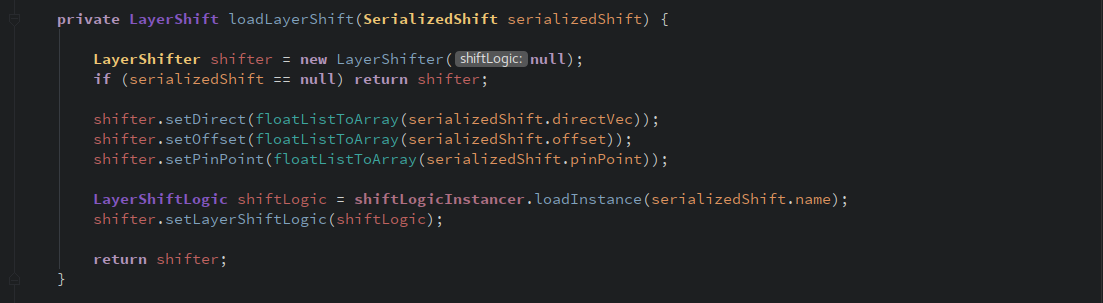
\includegraphics[width=1.2\linewidth]{img/8.png} 
  	\label{img:8} 
\end{center}

\subsection{Интсанцирование}
Инастанцирование производится по потому же принципу что и загрузка аттрибутов, с той лишь разницей, что метод отмеченный аннотацией \textit{\textbf{@EscapyInstanced("...")}}
не имеет аргументов. 
\begin{center}
	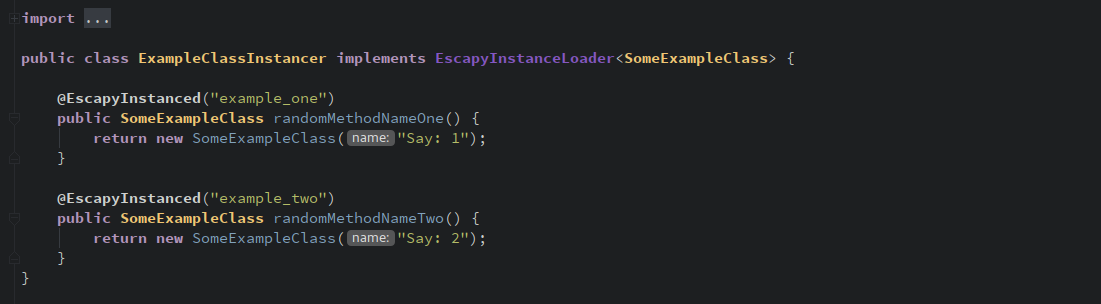
\includegraphics[width=1.2\linewidth]{img/14.png} 
  	\label{img:14} 
\end{center}
В свою очередь создание инстанции нужного нам объекта происходит через вызов метода:\\ \textit{\textbf{loadInstance(String: instanceName, Object[]: args);}} \\
или просто: \\  \textit{\textbf{loadInstance(String: instanceName);}} 
\begin{center}
	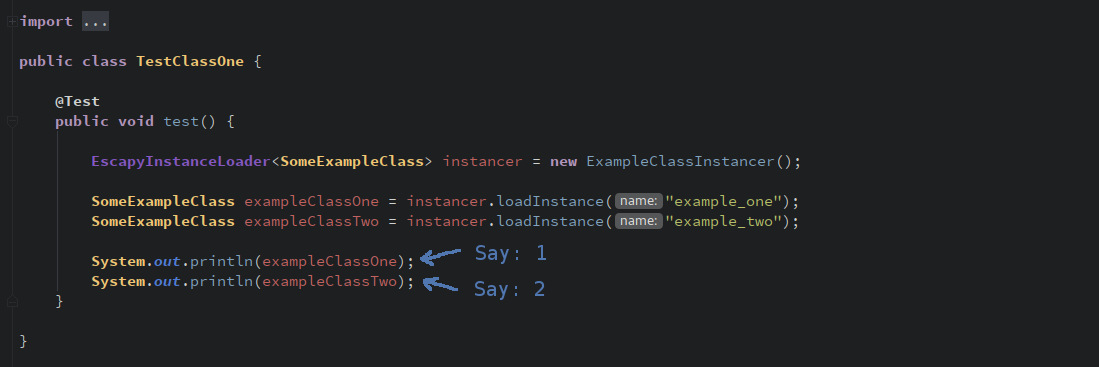
\includegraphics[width=1.2\linewidth]{img/15.png} 
  	\label{img:15} 
\end{center}


\chapter{Desktop}
На данный момент, этот пакет служит только для загрузки начальной конфигурации из json файла в desktop-версии приложений. Для этого используются такие интерфейсы (их реализации) как \textit{\textbf{DesktopConfigLoader и DesktopConfigLoaderBuilder}}. Очевидный пример использования этого пакета продемонстрирован в самом начале документа.
\begin{center}
	
\includegraphics[width=1.25\linewidth]{img/1.png} 
  	\label{img:9}
\end{center}
Builder создает нужную нам инстанцию загрузчика, после чего остается вызвать на этой инстанции метод <<\textit{\textbf{loadDesktopConfig();}}>> который заинстанцирует нужный нам объект и устновит в нем значения полей считанные из json файла.

\chapter{Graphic}
Пакет Graphic состоит из трех субпакетов: \begin{itemize*}
	\item \textit{\textbf{Camera}}
	\item \textit{\textbf{Render}}
	\item \textit{\textbf{Screen}}
\end{itemize*}
\section{EscapyCamera}
Класс из пакета \textit{\textbf{Camera}} инкапсулирующий \textit{\textbf{OrtographicCamera}} с дополнительным функционалом - простота и удобство, рекомендуется к использованию.

\section{Render}
Ключевой субпакет, на данный момент состоит из субпакетов: \begin{itemize*}
	\item \textit{\textbf{Fbo}}
	\item \textit{\textbf{Light}}
	\item \textit{\textbf{Mapping}}
	\item \textit{\textbf{Program}}
	\\
\end{itemize*}

\subsection{Mapping}
Данный пакет включает в себя 4 интерфейса, три из них содержат методы вызываемые во время отрисовки: \begin{itemize*}
	\item \textit{\textbf{GraphicRenderer}} - методы этого интерфейса вызываются во время 		отрисовки цветных(обычных) текстур объектов.
	\item \textit{\textbf{NormalMapRenderer}} - методы вызываются во время отрисовки 			текстур карты нормалей.
	\item \textit{\textbf{LightMapRenderer}} - методы вызываются во время отрисовки 			текстур карты света.
	\item \textit{\textbf{EscapyRenderable}} - этот интерфейс наследуется от трех выше 			перечисленных.
\end{itemize*}

\subsection{FBO}
FBO - иначе Frame Buffer Object, в движке представлен интерфейсом \textit{\textbf{EscapyFBO}} и его стандартной реализацией \textit{\textbf{EscapyFrameBuffer}} которая инкапсулирует \textit{\textbf{FrameBuffer}} из библиотеки libGDX, но с дополнительным полезным и удобным функционалом. О том как работают FrameBuffer'ы следует ознакомится самостоятельно через материалы посвященные \textit{\textbf{openGL}}.\\
\subsection{Program}
Cостоит из двух субпакетов \textit{\textbf{gl10}} и \textit{\textbf{gl20}}.
Первый использует нативные вызовы openGL без шейдеров в процессе рендеринга, второй в свою очередь нацелен на использование именно шейдеров.
\subsubsection{GL10} 
Функционалом gl10 пользуются такие классы как например: \begin{itemize*}
	\item \textit{\textbf{EscapyGLBlendRenderer}} - интерфейс ответственный за блендинг.
	\item \textit{\textbf{NativeSeparateBlendRenderer}} - нативная реализация интерфейса 		выше
	\item \textit{\textbf{LightMask}} - маска, используется для затемнения активной 			области экрана.
\end{itemize*}
\subsubsection{GL20} 
Пакет направленный на работу с шейдерами удобным способом. Работа осуществляется посредством двух основных интерфейсов \textit{\textbf{EscapyShader}} и \textit{\textbf{UniformsProvider}}, а так же интерфейсов от них налседующихся как \textit{\textbf{EscapySingleSourceShader}} и \textit{\textbf{EscapyMultiSourceShader}}.
Работа с юниформами (их загрузка и тп) осуществляется посредством вспомогательного класса \textit{\textbf{StandardUniforms}} и \textit{\textbf{Uniform<T>}} внутри него. 
\begin{center}
	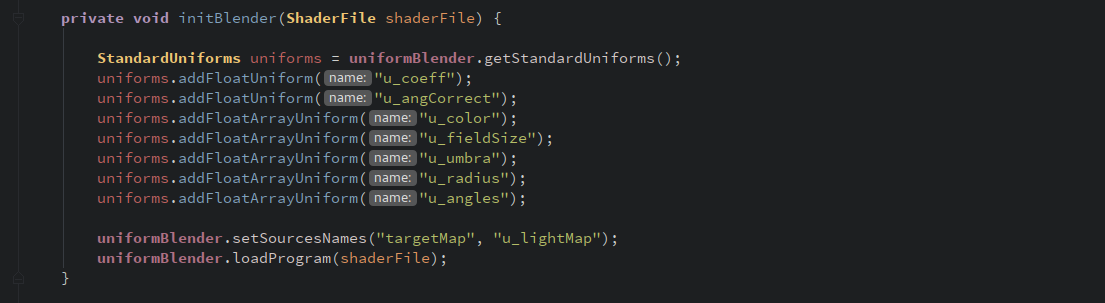
\includegraphics[width=1.2\linewidth]{img/9.png} 
  	\label{img:9} 
\end{center}
Выше изображен пример использования класса \textit{\textbf{StandardUniforms}}.

\newpage
В целом для работы с шейдерами достаточно двух стандартных реализаций интерфейсов
\textit{\textbf{EscapyUniformSingle}} и \textit{\textbf{EscapyUniformBlender}}. Их реализации предоставленные движком это \textit{\textbf{SingleRendererExtended}} и \textit{\textbf{BlendRendererExtended}} соотвественно. Достаточно в аргументах конструктора этих классов указать файлы .vert и .frag шейдеров, а с помощью метода 
\textit{\textbf{getStandardUniforms()}} установить значения для юинформов. Хорошим примером может послужить исходный код класса \textit{\textbf{EscapyLightSource}}.
\\
\subsection{Light}
Данный пакет как можно догадаться из названия служит работе со светом. 
\\Cубпакет \textit{\textbf{source}} отвечает за создание источников света с помощью классов  \textit{\textbf{EscapyLightSource}} и \textit{\textbf{LightSource}} (рекомендуется использовать второй). Субпакет \textit{\textbf{processor}} оветчает за правильную отрисовку источников света посредством интерфейса \textit{\textbf{EscapyLightProcessor}} и его двух стандартных реализаций \textit{\textbf{EscapyFlatLight}} и \textit{\textbf{EscapyVolumeLight}} их ключевое отличие заключается в использовании карты нормалей, в первом случае оная не используется и свет получается плоским как и следует из описания.
\begin{center}
	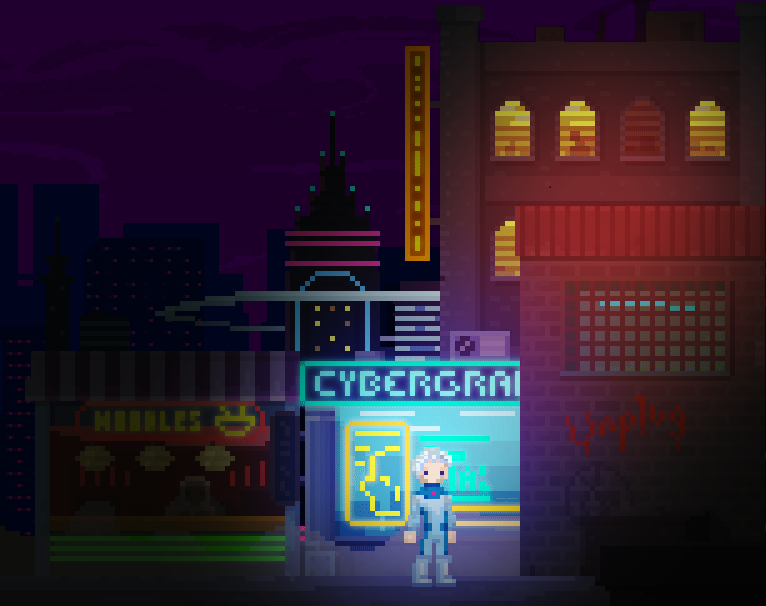
\includegraphics[width=1\linewidth]{img/10.png}
	Пример с объемным светом.
	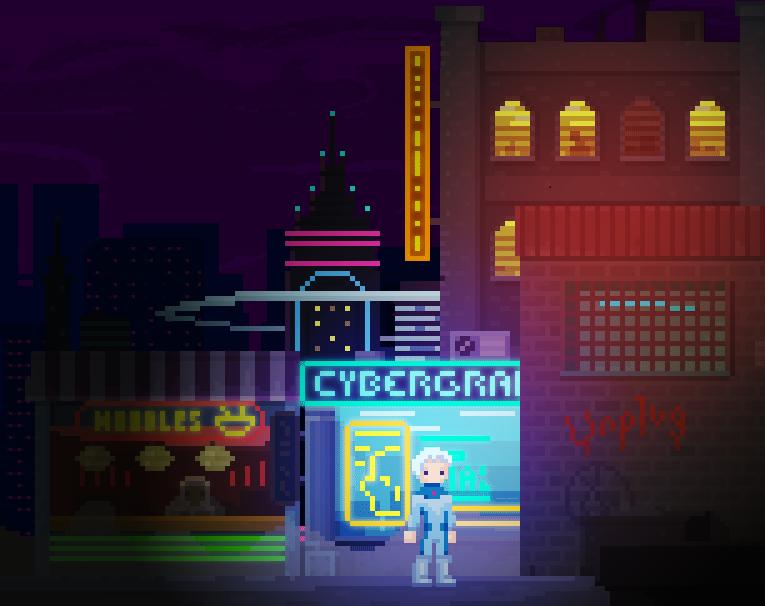
\includegraphics[width=1\linewidth]{img/11.png}  
	Пример с плоским светом.
  	\label{img:1011} 
\end{center}

\chapter{Group}
Данный пакет предназначен для упрощения работы с игровыми объектами на всех этапах их жизни посредством конфигурационных файлов (в стандартной реализации движка это json). На данный момент этот пакет представлен тремя субпакетами: \begin{itemize*}

	\item \textit{\textbf{map}} - отвественный за игровые объекты
	\item \textit{\textbf{render}} - ответсвенный за процесс отрисовки объектов
	\item \textit{\textbf{container}} - отвественный за делегирование первых двух
	
\end{itemize*}
\section{Container}
Представлен тремя основными интерфейсами, а так же их реализациями по умолчанию посредством которых осуществляется работа. Интерфейсы вместе с имплементриующими классами:
\begin{itemize*}
	\item \textit{\textbf{(I) EscapyGroupContainer: (C) DefaultGroupContainer}}
	\item \textit{\textbf{(I) EscapyLocationContainer: (C) DefaultLocationContainer}}
	\item \textit{\textbf{(I) EscapyRendererContainer: (C) DefaultRendererContainer}}
\end{itemize*}
Классы \textit{\textbf{DefaultLocationContainer}} и \textit{\textbf{DefaultRendererContainer}} имеют конструкторы с модификатором доступа \textit{\textbf{protected}} потому их невозможно заинстанцировать на прямую, вместо этого надо использовать класс \textit{\textbf{DefaultGroupContainer}}.
\subsection{DefaultGroupContainer}
Основной класс контейнера объектов реализующий интерфейс \textit{\textbf{EscapyGroupContainer}} от которого содержит метод \textit{\textbf{boolean initialize();}}, который следует самостоятельно и однократно за весь жизненный цикл приложения, вызвать во время инициализации оного.
\begin{center}
	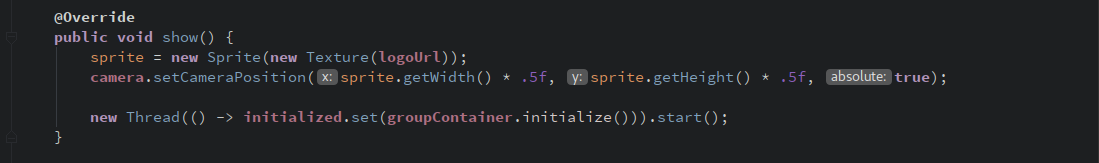
\includegraphics[width=1.2\linewidth]{img/12.png} 
  	\label{img:120} 
  	Пример вызова метода в новом потоке во время стартового экрана приложения.
\end{center}

\subsection{Сериализация}
В случае с классом \textit{\textbf{DefaultGroupContainer}} для сериализации используется json файл который имеет следующую структуру: 
\begin{center}
	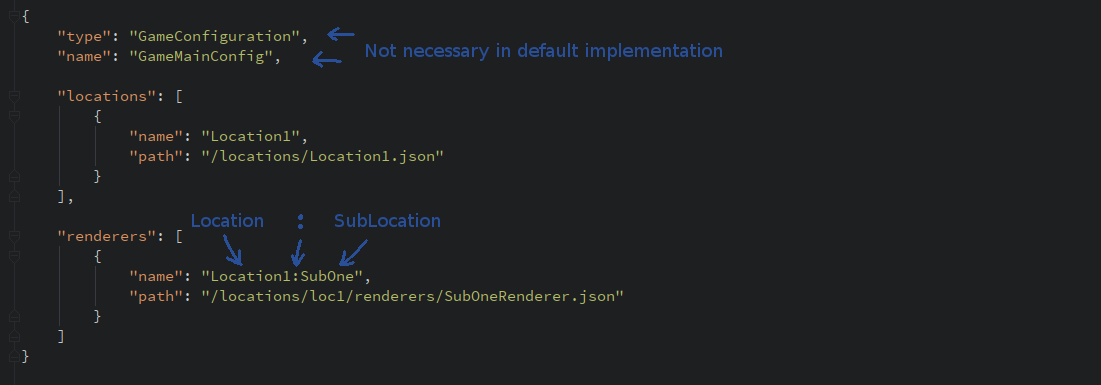
\includegraphics[width=1.2\linewidth]{img/13.png} 
  	\label{img:130} 
\end{center} 
В массиве \textit{\textbf{locations}} следует указать имя и путь к файлу из которой должна загружаться локация, в массиве \textit{\textbf{renderers}} так же следует указать путь файла из которого будет загружатся \textit{\textbf{renderer}}, однако имя должно содержать 
название локации и имя сублокации для \textit{\textbf{renderer'a}} разделенное двоеточием.\\ В конструкторе \textit{\textbf{DefaultGroupContainer}} следует указать путь на json файл объекта, а так же загрузчики \textit{\textbf{DefaultLocationLoader}} и \textit{\textbf{DefaultRendererLoader}}
\begin{center}
	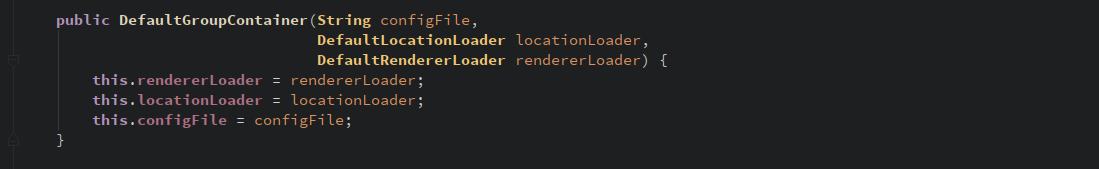
\includegraphics[width=1.2\linewidth]{img/16.png} 
  	\label{img:160} 
\end{center} 
Для создания инстанций загрузчиков рекомендуется использовать предназначенные для этого строители: \textit{\textbf{DefaultLocationLoaderBuilder}} и \textit{\textbf{DefaultRendererLoaderBuilder}}.
 
\newpage
\section{Map}
Этот субпакет отвечает за игровые объекты, он представлен основными интерфейсами:
\begin{itemize*} 
	\item \textit{\textbf{EscapyLocation}} - интерфейс основной локации
	\item \textit{\textbf{EscapySubLocation}} - интерфейс сублокации внутри основной 			локации
	\item \textit{\textbf{EscapyLayer}} - интерфейс слоев внутри сублокации
	\item \textit{\textbf{EscapyLayerShift}} - интерфейс смещения слоя
	\item \textit{\textbf{EscapyLayerShiftLogic}} - интерфейс логики смещения слоя
	\item \textit{\textbf{EscapyGameObject}} - интерфейс игровых объектов внутри слоев
	\item \textit{\textbf{EscapyGameObjectRenderer}} - интерфейс рендерера игровых 				объектов
	\\
\end{itemize*}
\subsection{DefaultLocationLoaderBuilder}
Каждый из вышеперечисленных интерфейсов имеет свою имплементацию по умолчанию, и что бы собрать их вместе в одну целую и рабочую группу следует воспользоваться строителем 
\textit{\textbf{DefaultLocationLoaderBuilder}} который создаст инстанцию имплементирующую 
\textit{\textbf{DefaultLocationLoader}} которая в свою очередь сможет загрузить локацию из json файла. При создании объекта класса \textit{\textbf{DefaultLocationLoader}}, тот в конструкторе получает инстанцию очередного загрузчика \textit{\textbf{DefaultSubLocationLoader}}, а тот в свою очередь 
инстанцию \textit{\textbf{DefaultGameObjectLoader}}. \\\\
В целом это выглядит следующим образом: 
\begin{itemize*}
	\item \textit{\textbf{DefaultLocationLoader}}
	\begin{itemize*}
		
		\item \textit{\textbf{DefaultSubLocationLoader}}
		\begin{itemize*}
			\item \textit{\textbf{subLocationLayerShiftLogicAttributeLoader}}
			\item \textit{\textbf{subLocationLayerAttributeLoader}}
			\item \textit{\textbf{subLocationAttributeLoader}}
			\item \textit{\textbf{DefaultGameObjectLoader}}
			\begin{itemize*}
				\item \textit{\textbf{gameObjectAttributeLoader}}
			\end{itemize*}
		\end{itemize*}
		\item \textit{\textbf{locationAttributeLoader}}
		\\
	\end{itemize*}
\end{itemize*}
Как можно заметить в конструктор основных загрузчиков так же передаются загрузчики аттрибутов обозначенных в json файле полем-массивом \textit{\textbf{"attributes": [...]}}, эти загрузчики являются имплементациями \textit{\textbf{EscapyInstanceLoader<T>}}.

\newpage
\subsection{Cериализация}
Пример ниже иллюстрирует как должен выглядить минимальный полный json файл конфигурирующий станартную реализацию игровой \textit{\textbf{сублокации}}.
\begin{center}
	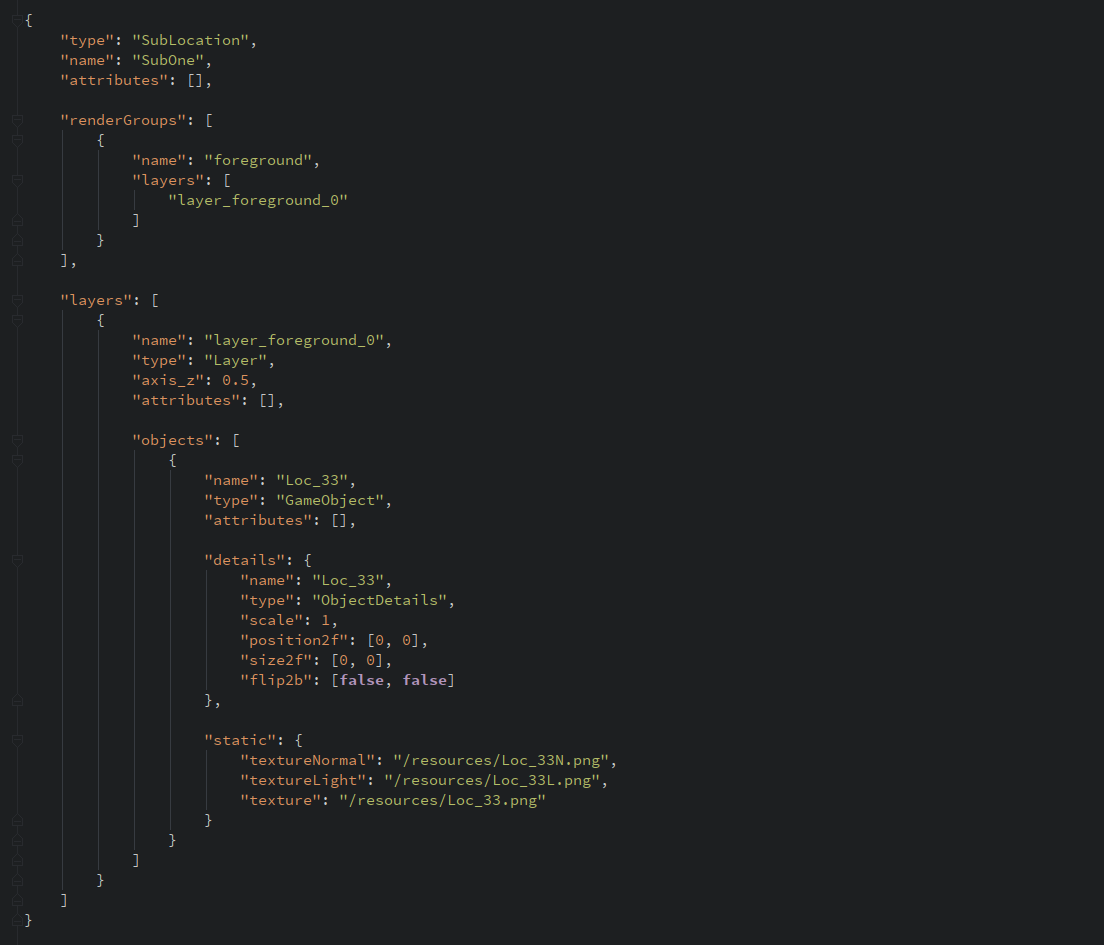
\includegraphics[width=1.2\linewidth]{img/21.png} 
  	\label{img:210} 
\end{center} 

\subsection{EscapyLocation}
Стандартной имплементацией интерфейса \textit{\textbf{EscapyLocation}} является класс под названием \textit{\textbf{Location}}, который загружается из простого json файла вида:
\begin{center}
	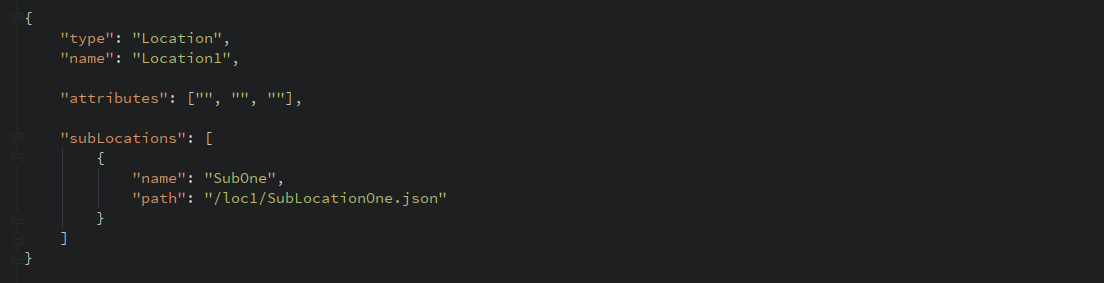
\includegraphics[width=1.2\linewidth]{img/17.png} 
  	\label{img:170} 
\end{center} 
\subsection{EscapySubLocation}
Сублокации за котороые отвечает интерфейс \textit{\textbf{EscapySubLocation}} и его стандартная имплементация \textit{\textbf{SubLocation}} загружаются из json файла вида:
\begin{center}
	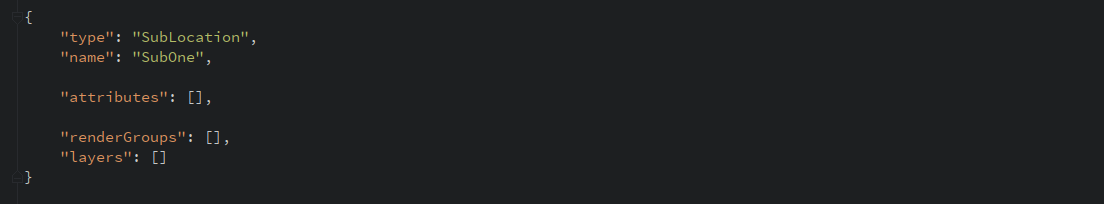
\includegraphics[width=1.2\linewidth]{img/18.png} 
  	\label{img:180} 
\end{center} 
\subsection{RenderGroups}
Массив \textit{\textbf{"renderGroups"}} содержит массив слоев, которые будут отрисовываться на графическом конвейере в таком порядке в каком они расположенны в массиве. 
\begin{center}
	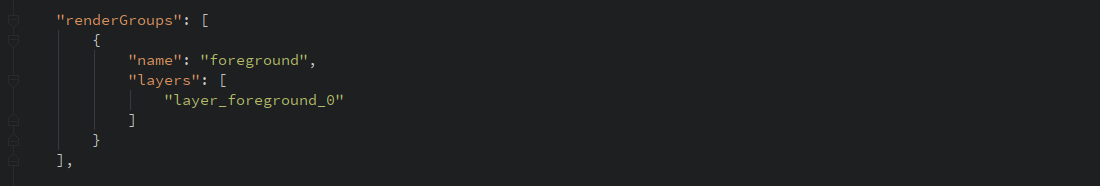
\includegraphics[width=1.2\linewidth]{img/19.png} 
  	\label{img:190} 
\end{center} 
\subsection{Layers}
Массив \textit{\textbf{"layers"}} это массив слоев, каждый из которых помимо стандартных полей унаследованных от шаблона \textit{\textbf{EscapySerialized}}, содержит уникальное поле \textit{\textbf{"axis\_z"}} определяющее позицию слоя на оси Z. Так же каждый из слоев содержит поле \textit{\textbf{shift}} хранящее информацию о смещении слоя и массив игровых объектов \textit{\textbf{"objects"}}
\begin{center}
	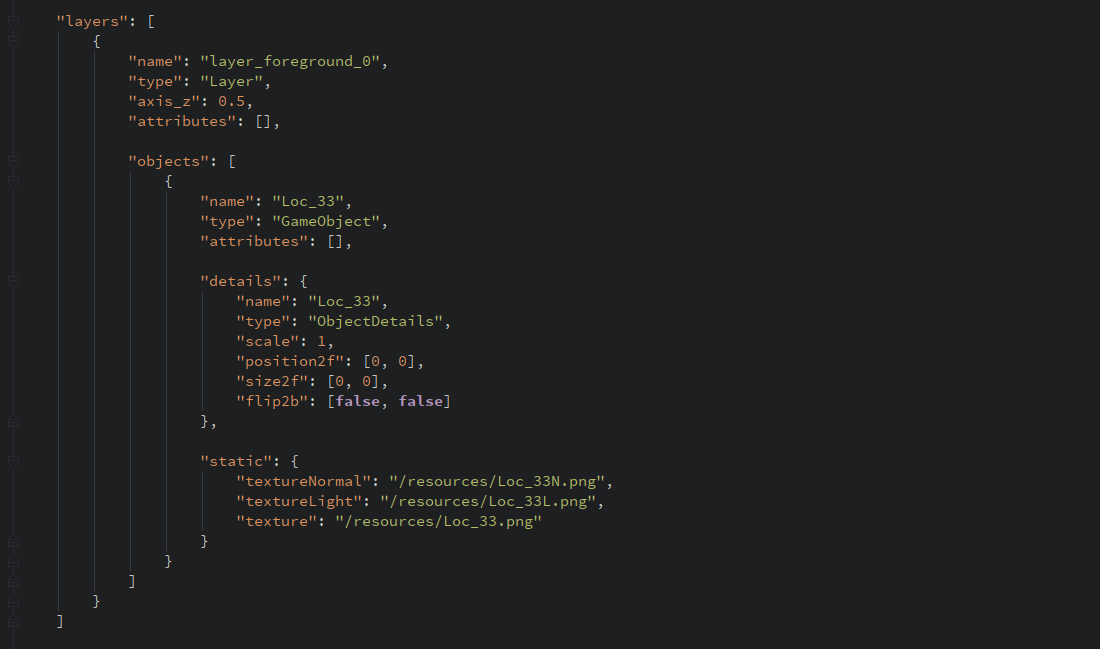
\includegraphics[width=1.2\linewidth]{img/20.png} 
  	\label{img:200} 
\end{center} 
Каждый из таких объектов содержит поля унаследованные от \textit{\textbf{EscapySerilized}}, а так же поле \textit{\textbf{"details"}} содержащее информацию об объекте, здесь стоит обратить внимание на то, что поле \textit{\textbf{"name"}} из \textit{\textbf{"details"}} переопределяет значение аналогичного поля самого объекта.
\subsubsection{Static, dynamic, etc?}
На данный момент в движке представленны только статические объекты (не имеющие какой либо анимации и т.п.), потому у игрового объекта есть только поле \textit{\textbf{"static"}} с путями к файлам текстур, однако в будщем это изменится.

\newpage
\section{Render}
Задача этого субпакета заключается, как следует из названия в отрисовке игровых объектов, а так же разнообразных источников света и т.п. Все вышеописанное выполняется посредством одного интерфейса \textit{\textbf{EscapyRenderer}}, а так же его имплемантации по умолчанию - \textit{\textbf{DefaultRenderer}}. Интерфейс содержит три ключевых метода:

\begin{itemize*}
	\item \textit{\textbf{void render(float delta);}}
	\item \textit{\textbf{void resize(int width, int height);}}
	\item \textit{\textbf{<T> T getRendererAttribute(String name);}}
\end{itemize*}
Последний из вышеперечисленных методов стандартной имплементации позволяет получать доступ ко всем объектам рендерера, а так же ко вложенным в них объектам с помощью оператора \textit{\textbf{":"}}
\begin{center}
	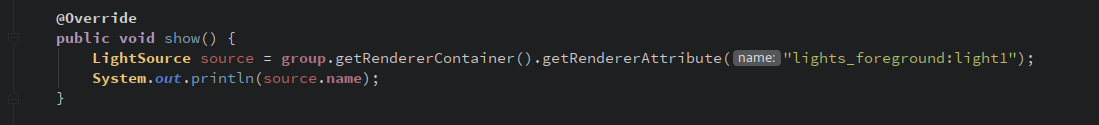
\includegraphics[width=1.2\linewidth]{img/22.png} 
  	\label{img:220} 
\end{center} 

\subsection{DefaultRendererLoaderBuilder}
Аналогично субпакету \textit{\textbf{Map}}, для комфортной работы с рендерером начиная с этапа его загрузки, следует воспользоваться строителем \textit{\textbf{DefaultRendererLoaderBuilder}} которой сам создаст инстанцию загрузчика \textit{\textbf{DefaultRendererLoader}}, а та в свою очередь загрузит нужный рендерер из json файла когда возникнет необходимость. Поскольку для сериализации используется Gson шаблон \textit{\textbf{EscapySerialized}}, который содержит массив с аттрибутами \textit{\textbf{"attributes"}}, то разумеется и загрузчик позволяет на обработку этих самых аттрибутов посредством механизма \textit{\textbf{EscapyInstanceLoader<T>}}.

\subsection{Сериализация}
Для (де)сериализации рендерера используется следующий шаблон:
\begin{center}
	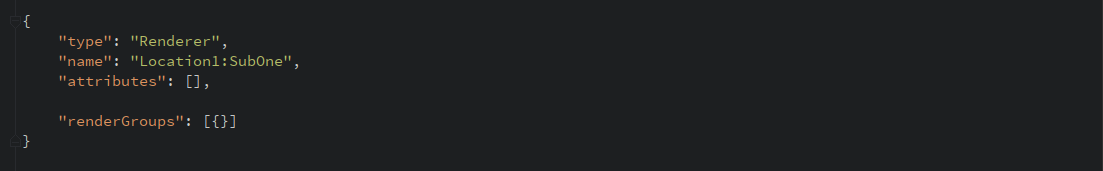
\includegraphics[width=1.2\linewidth]{img/23.png} 
  	\label{img:230} 
\end{center} 

\subsection{RenderGroups}

\end{document}



